\section{FPGA}
This section will present an overview of the various components that need to be developed throughout this project.
In particular, the components that are specific to this application will be discussed in more detail.
See figure \ref{fig:fpga} for a view of the components.

\begin{figure}[H]
	\centering
	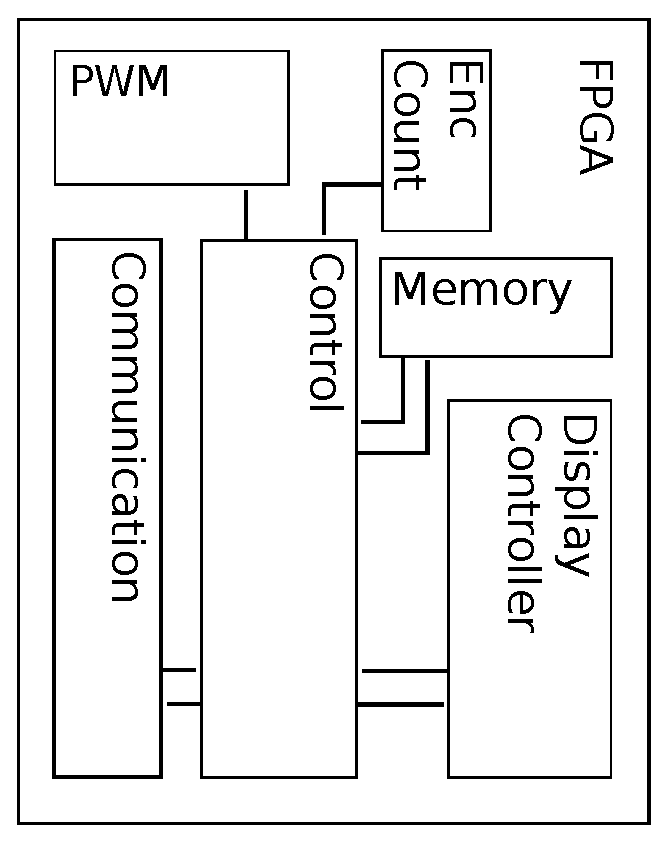
\includegraphics[angle=90,width=.5\linewidth]{images/fpga_block}
	\caption{An overview of the components to be written in VHDL.}
	\label{fig:fpga}
\end{figure}

\subsection{Communication}
This block will maintain the communication link with the PC.
As mentioned in previous sections, only one image is stored on the FPGA at any time.
This means that displaying a sequence of images has to be done by continuously rewriting the image present on the FPGA.
The communication will be done using $\mu$TosNet.
According to \cite{utosnet} $\mu$TosNet is capable of data rates of 10 Mbps.
Since each image is a known size of $40\times40\times12$ bits or 0.0192 Mbps, this would allow for transferring up to approximately 520 images per second.

\subsection{Enc. Count}
This block is responsible for calculating the current position of the motor.
It does this by monitoring the output of the photo sensor.
The photo sensor generates 16 pulses for each revolution of the motor.
This allows for a resolution of 22.5$^\circ$.
This is insufficient since an update is made every 2$^\circ$.
In order to artificially increase the resolution the time, $\Delta$t between each pulse is measured.
This makes it possible to estimate the time per degree by $t_d = \frac{\Delta\text{t}}{22.5^\circ}$.
Estimation of the angular position between pulses is then simply a matter of adding a degree to the position every $t_d$ seconds.
Both $t_d$ and the angular position are output from the block.

\subsection{PWM}
In order to keep the motor spinning at a constant velocity, it is necessary to continuously adjust the PWM used to control the motor.
Assuming a speed of 2200 RPM or $\approx$37 Hz as the goal, this results in $37\cdot360=13320$deg/sec.
This a a target $t_d$ of $\frac{1}{13320}=7.75\cdot10^{-5}$s.
The block will read the $t_d$ output from the enc. count block and adjust the PWM in order to minimize $|t_{d target}-t_d|$.

\subsection{Control}
This block is the connection point between all of the other blocks.
In an effort to simplify communication between blocks it was decided to create this block as a mediator.

\subsection{Memory}
The image to be stored consists of 40$\times$40 pixels, Each pixel consist of $4 \cdot 3 = 12$ bits.
An image therefore requires 40$\times$40$\times$12   =  19,200 kb to store.  
Since this memory block will be used only for lookups, it would use unnecessary amounts of logic to create a 2D array representation on the FPGA.
For this reason, it would be desirable to store the image in block RAM.
The information stored in RAM can then be accessed given the address location.
Block RAM is synchronous such that when a write or read is requested, it will be executed on the next clock event.
The delay involved with reading and writing to and from memory is insignificant in this application, as the FPGA provides a 50 MHz clock, which is significantly higher than the rate at which a new line is to be displayed.
The block RAM on the FPGA used for this project is 54 kb, which is more than enough to store the image. \cite{FPGA}

\subsection{Display controller}
This block converts the information stored in the matrix image to PWM signals necessary to drive the LEDs.

The encoder outputs the current angular position of the motor.
The matrix uses this position to determine which line should be generated.
A line contains 20 pixels.
Each pixel is described with 12 bits, 4 bits for each colour channel.
These 4 bits determine the duty cycle of the PWM used to drive that channel.

The controller retrieves these 20 "pixel descriptions" and converts them to packets of 64 bits.
In each packet the 4 LSBs are redundant but will be set to zero to avoid floating pins.
The remaining 60 bits contain information about the state of each channel at that time.
By continuously updating these sets, each bit will create a PWM for its respective LED.
The frequency of the signal is set based on the rotational velocity of the motor.

The motor with gearing rotates at 2200 RPM which gives a frequency of 37 Hz.	
For each revolution the display controller is expected to provide 180 updates, an update per 2$^\circ$.
This results in:

$$37 \cdot 180 = 6660 ~\text{updates/sec}$$

Each update should therefore occur with a time step of $\frac{1}{6660} = 0.00015s$ Which provides aa lower limit for what the PWM frequency should be.  \\

As the LED driver component (CAT4016) has a limit of 25 Mhz, and each update consists of latching 64 bits to the LED, this creates a possible bandwidth of $$\frac{25000000}{64} =  390625 Hz$$. 
As the LED itself cannot process 64 bits faster than this, this will be set as the upper limit for the PWM frequency.    
$$6667 \text{Hz}  \leq \text{PWM - Frequency}  \leq 390625 \text{Hz}  $$

It was determined to use a PWM - frequency of 20 kHz, as this lies within the range, and allow for some deviations within the range.  \\

Each duty cycle of the PWM signal consists of 10$\times$64 bit packets.
Thereby each packet is sent with an interval of $5 \cdot 10^{-6}$
While a higher resolution would be desirable, this would lead to a higher bandwidth requirement than what is available.
At $10\times64$ bit packets per duty cycle, allowing for 10\% resolution on the PWM frequency, a total of 51\% of the available bandwidth is used.
Having 5\% resolution, for instance, would require 102.4\% of the available bandwidth.

